% ------------------------------------------------------ %
% 由于很多参加数学建模竞赛的同学没有\LaTeX基础,因此做
% 本模板用于各位写手快速上手写作,不要追究原理,先把模
% 板用会再说。PS:上交附件时请把这部分注释全部删掉,作
% 品出现任何信息都会判为作弊,这里出现我的信息了。
% ------------------------------------------------------ %
%         谈欣 如有错误请联系1792733991@qq.com
%         谈欣 如有错误请联系1792733991@qq.com
%         谈欣 如有错误请联系1792733991@qq.com
% ------------------------------------------------------ %
%     更多内容关注:
%     个人网页:https://jack-tanxin.github.io
%     个人Github主页:https://github.com/Jack-TanXin
% ------------------------------------------------------ %
% 数学建模论文是个结构非常复杂的论文,因此使用\LaTeX必须
% 编译数次——无论你使用哪种发行版或编辑器,原因详见\LaTeX
% 的编译原理,一般写好以后编译2次就是文章真正的面目。
% ------------------------------------------------------ %
%              请使用XeLaTeX进行编译!!!
%              请使用XeLaTeX进行编译!!!
%              请使用XeLaTeX进行编译!!!
% ------------------------------------------------------ %
\documentclass[UTF8,12pt]{ctexart}

% ------------------------------------------------------ %
% 下面的包基本上都是数学建模必需的包,没有这些包我想基
% 本上是写不出完整的论文的,仅供大家参考
% ------------------------------------------------------ %
\usepackage[a4paper,left=2.5cm,right=2.5cm,top=2.5cm,bottom=2.5cm]{geometry}    % 这个包专门用来调整页边距
\usepackage{amsmath}    % 数学包
\usepackage{fancyhdr}   % 页眉页脚设定

% 插入图片的包
\usepackage{graphicx}
\usepackage{subfigure}

% 插入表格的包
\usepackage{float}
\usepackage{booktabs}

% 颜色包,定义颜色,会在附录中使用到
\usepackage{xcolor}
\definecolor{gray}{RGB}{128,128,128}

% 链接包:这个宏包在论文中没有任何作用,单纯为了方便给我做广告
% 让目录可以索引到正文,所以这个包不能删!
\usepackage{hyperref}
\hypersetup{colorlinks=true,linkcolor=black,citecolor=blue,filecolor=black,urlcolor=cyan,pdftitle={Overleaf Example},pdfpagemode=FullScreen}
    
% 附录插入代码
\usepackage{listings}
\lstset{basicstyle=\ttfamily,columns=fullflexible,frame=single,breaklines=true,keywordstyle=\color{blue},commentstyle=\color{gray}}

% 务必注意:图片在figures目录下
% 务必注意:图片在figures目录下
% 务必注意:图片在figures目录下
\graphicspath{{figures/}} 



\begin{document}   % 文章开始



% ----------------------------------------------- %
%              请在这里输入文章标题
% ----------------------------------------------- %
%              请在这里输入文章标题
% ----------------------------------------------- %
\title{数学建模内容参考模板}



\author{} % 不要动!!
\date{} % 不要动!!
\maketitle % 不要动!!
\vspace{-4em}  % 不要动!!



% ---------------------------------------------------- %
%  打开chapter文件夹里的摘要.tex文件,编辑其中的内容
% ---------------------------------------------------- %
%  打开chapter文件夹里的摘要.tex文件,编辑其中的内容
% ---------------------------------------------------- %
\begin{abstract}

    摘要是全文最重要的部分,也是阅卷人首先看到的部分,阅卷人会只根据摘要将文章分成三六九等,所以如果不认真写摘要的话你就会有大麻烦,请务必留至少两小时用于摘要的打磨,将其控制在1面!!!
    
    针对问题一:在写摘要的时候请搞清楚,首先摘要的第一段是题设的背景,你需要随便胡扯几句,但别扯太多,毕竟要把摘要控制在一面很难!然后写完第一段后从第二段开始就要开始介绍你对每个题目的理解、过程以及求解与评价,语言尽量精炼,不要啰嗦,再强调一次:那么多内容的摘要压缩在一面非常难!下面我将给大家演示如何对于自己已经完成的“模型建立与求解”部分进行摘要描述。
    
    针对问题二,本文基于可视化和假设检验对所给数据集进行数据分析。首先对产品的销售价格和销售量的关系进行探究,本文分别通过\textbf{斯皮尔曼相关系数}对相关性进行定量描述,求得$\rho$=-0.2946,反映出\textbf{销售价格和销售量的相关性较弱}。接着对区域与销量的关系进行探究,通过\textbf{方差检验}得知\textbf{不同地区对订单的需求量有显著差异},并通过直方图探究出不同区域产品的需求量的不同特性。然后,本文对产品的销售方式与需求量的关系进行探究,通过\textbf{Mann-Whitney U}检验得出\textbf{线上销售与线下销售的销售量存在显著差异}。最后,通过\textbf{单样本Wilcoxon符号秩检验}将时间序列整体与促销活动单日的销量相比较,得出\textbf{促销活动单日的销量与平时的销量有显著差异}。为了将各特征的分布以及定量分析所得出的结论直观化,本文利用小提琴图、箱线图、直方图等对相关特征进行可视化,结果与定量分析一致。
    
    针对问题三,摘要内容摘要内容摘要内容摘要内容摘要内容摘要内容摘要内容摘要内容摘要内容摘要内容摘要内容摘要内容摘要内容摘要内容摘要内容摘要内容摘要内容摘要内容摘要内容摘要内容摘要内容摘要内容摘要内容摘要内容摘要内容摘要内容摘要内容摘要内容摘要内容摘要内容摘要内容摘要内容摘要内容摘要内容摘要内容摘要内容摘要内容摘要内容摘要内容摘要内容摘要内容摘要内容摘要内容摘要内容摘要内容摘要内容摘要内容摘要内容摘要内容摘要内容摘要内容摘要内容摘要内容摘要内容摘要内容摘要内容摘要内容。
    
    第二部分分别是针对数据分析的任务和机器学习的任务,可以看到摘要第一句话用于概括整个小题大致是怎么做的,从第二句话开始展开每一步,用“首先”、“接着”、“然后”、“最后”依次描述。在摘要中务必要把你的结果和评价情况直接呈现出来并且加粗,同时你使用的关键方法也需要加粗,通过这个源文件相信你已经知道该如何加粗了。
    
    \vspace{1em} % 移除2个行距的空白:这句代码千万不能动!!!移除2个行距的空白:这句代码千万不能动!!!
    
    \noindent{\textbf{关键词:}随机森林;方差选择法;Voting Classifier;层次聚类分析;决策树}
    
\end{abstract} 



\thispagestyle{empty}  % 清除摘要页的页码,不要动!!
\newpage  % 另开一页写目录,不要动!!



% ------------------------------------------------------------ %
%    这一部分自动生成目录,同时清除目录页的页眉和页脚,
%    清除目录页的页码以保证正文的第一面为页码1
%    并新开一面,如果不想要目录直接删除这部分
% ------------------------------------------------------------ %
\pagestyle{fancy}
\fancyhead{} % 页眉清空
\fancyfoot{} % 页脚清空
\begin{center} \tableofcontents \end{center} 
\thispagestyle{empty}\newpage



% ------------------------------------------------------------ %
%    设置正文的页眉、页脚,页眉没有内容,页码在页脚中间
%    并将本页设置为第一页
%    我浅浅用页眉给自己做了个广告,大家记得删除啊!
% ------------------------------------------------------------ %
\pagestyle{fancy} % 不要动!!
% 这是个广告,正式使用时请删除这一行
\fancyhead[R]{\href{https://jack-tanxin.github.io}{进入我的个人网页}} 
% 删除上一行后将下面的这句\fancyhead[R]{}前面的百分号删除就行
% \fancyhead[R]{}
\fancyhead[C]{} % 页眉中间清空 不要动!!
\fancyhead[L]{} % 页眉左侧清空 不要动!!
\fancyfoot[R]{} % 页脚右侧清空 不要动!!
\fancyfoot[C]{- {\thepage}\ -} % 页脚中间为页码 不要动!!
\fancyfoot[L]{} % 页脚左侧清空 不要动!!
\setcounter{page}{1}  % 不要动!!



% ---------------------------------------------------------- %
% 接下来的部分即为文章每个章节的内容,我这里使用的是2022年
% 国赛的论文,当时是有四道题目,每次竞赛的题目量都不一定,
% 请酌情更改,另外有时候可能会多一个灵敏度分析或是其他创新
% 的内容,记住一个准则:有多少个章节就在chapter文件夹中制作
% 多少个tex文件,每个文件夹管一个章节就行啦!!!
% ---------------------------------------------------------- %



% ---------------------------------------------------------- %
%    打开chapter文件夹里的问题重述.tex文件,编辑其中的内容
% ---------------------------------------------------------- %
%    打开chapter文件夹里的问题重述.tex文件,编辑其中的内容
% ---------------------------------------------------------- %
\section{问题重述}

\subsection{问题背景}

数学建模比赛论文是要我们解决一道给定的问题,所以正文部分一般应从问题重述开始,一般确定选题后就可以开始写这一部分了。
这部分的内容是将原问题进行整理,将问题背景和题目分开陈述即可,所以基本没啥难度。
本部分的目的是要吸引读者读下去,所以文字不可冗长,内容选择不要过于分散、琐碎,措辞要精练。
注意:在写这部分的内容时,绝对不可照抄原题!(论文会查重)
应为:在仔细理解了问题的基础上\cite{ref1},用自己的语言重新将问题描述一遍。语言需要简明扼要,没有必要像原题一样面面俱到。


\subsection{问题提出}

看到上面插入的“\cite{ref1}”了吗,这是在引用后面的文献,所以大家在文中引用文献的时候也像我这样在句子结束后面加一个这个就行了,他是蓝色的,比较醒目,一般也都是蓝色的好像。

现有一组由专家给出的关于玻璃的数据,要求通过分析与建模解决下面若干问题:

\textbf{问题1:} 问题提出内容问题提出内容问题提出内容问题提出内容问题提出内容问题提出内容问题提出内容问题提出内容。

\textbf{问题2:} 问题提出内容问题提出内容问题提出内容问题提出内容问题提出内容问题提出内容问题提出内容问题提出内容问题提出内容。

\textbf{问题3:} 问题提出内容问题提出内容问题提出内容问题提出内容问题提出内容问题提出内容问题提出内容问题提出内容问题提出内容。

\textbf{问题4:} 问题提出内容问题提出内容问题提出内容问题提出内容问题提出内容问题提出内容问题提出内容问题提出内容问题提出内容。



% ---------------------------------------------------------- %
%    打开chapter文件夹里的问题分析.tex文件,编辑其中的内容
% ---------------------------------------------------------- %
%    打开chapter文件夹里的问题分析.tex文件,编辑其中的内容
% ---------------------------------------------------------- %
\section{问题分析}

本文对于赛题题设,从多个角度对数据集进行统计分析与统计推断,本部分将对四个问题进行简要分析,同时赛题的每个问题的解答完整流程以流程图的形式在附录A给出。

\subsection{问题一的分析}

针对问题一,第一问要求关于术中、术后 24h 不良反应,判断新药组和原有药物组是否存在显著差异。首先对附件1中进行数据清洗、特征缩放、特征编码,由于不良反应在编码后均为分类特征,故用基于多变量可视化分析的定性方法和基于卡方检验的定量方法探究不同药组对于不良反应的差异性。

第二问要求建立一个有效的分类模型用于对患者的不良反应进行预判。本文基于经过数据预处理的数据集,首先对标签进行分布分析,并对标签比例严重失衡的数据集进行上采样处理。接着把数据按比例分为训练集和测试集。然后基于决策树对训练集进行特征提取,使用经过训练的决策树模型实现对两大类、8组不良反应的预判。最后基于混淆矩阵、ROC图对模型在测试集上的表现进行评价。


\subsection{问题二的分析}

针对问题二,第一问要求判断新药组和原有药物组在生命体征数据方面是否表现出显著差异。首先对数据进行数据清洗和特征编码。接着基于Spearman、Kendall相关性分析计算特征之间的相关性并删除相关性高特征之一,为避免高维数据集造成数据分析困难,基于主成分分析法在保留较高方差解释比例的前提下对数据进行降维。最后对降维后的特征进行正态性检验,分别基于独立样本t检验和Mann-Whitney U研究不同药组对生命体征数据的差异性。

第二问在第一问的基础上,探究造成新药对生命体征数据显著差异的影响因素。本文基于经过数据预处理的数据集,基于LightGBM对以受试者情况和病史为特征空间、以检验出显著差异的生命特征组为标签的数据集进行特征提取,在确保模型性能极好的前提下并利用树模型独有的特征重要性评价功能对各特征对标签的作用效果进行评价,最后利用条形统计图呈现。

\subsection{问题三的分析}

针对问题三,要求根据用药信息和患者信息预测对给药后 3 分钟以内的 IPI 数据。首先对数据进行数据清洗和特征编码。接着为了避免大量分类特征造成特征空间离散从而影响模型提取特征,基于主成分分析法对特征空间进行降维。然后基于岭回归和支持向量机回归分别对数据集进行特征提取,并用线性加权法对二者结果进行融合。最后为了提高模型的可靠性和准确性,本文基于MAE、MSE和数据扰动对模型在测试集上的表现和回归的稳定性进行评价。


\subsection{问题四的分析}

针对问题四,要求基于现有数据找出与术后满意度有关的因素,本文使用定性方法和定量方法分别进行模型求解。

基于斯皮尔曼、肯德尔相关性分析分别对数值特征和分类特征与术后满意度的相关性进行探究。首先对数据进行数据清洗,对分类特征进行特征编码,对数值特征进行特征缩放。接着对两类特征分别进行相关性分析,求得相关系数。最后用条形统计图对结果进行可视化,得出初步结论。

基于树模型的树状图对术后满意度划分的定量探究。首先对数据进行预处理,并将五维关于术后满意度的特征聚合为一维关于术后满意度的评分作为标签,为避免术后满意度评分分布不均衡导致模型难以提取特征,对数据集进行上采样。然后按比例将数据集划分为训练集和测试集,并基于随机森林对训练集进行特征提取。最后导出随机森林的树状图,并通过树状图获取分类的具体依据。


















% ---------------------------------------------------------- %
%    打开chapter文件夹里的模型假设.tex文件,编辑其中的内容
% ---------------------------------------------------------- %
%    打开chapter文件夹里的模型假设.tex文件,编辑其中的内容
% ---------------------------------------------------------- %
\section{模型假设}

% 这个地方开始涉及到顺序环境,也就是1,2,3……排序,每个序号一个\item,然后用\begin{enumerate}和\end{enumerate}包起来就可以

\begin{enumerate}
  \item 假设本文的数据真实可靠。
  \item 假设患者除了使用本题所用药物外,未使用其他药物。
  \item 假设患者出现的不良反应是除了环境等客观因素造成的。
  \item 本文认为所给的数据不存在过大的人为过失。
  \item 假设患者在用药前并未吃其他食物。
  \item 本文认为药物在存放过程中成分没有发生改变。
\end{enumerate} 



% ---------------------------------------------------------- %
%    打开chapter文件夹里的符号说明.tex文件,编辑其中的内容
% ---------------------------------------------------------- %
%    打开chapter文件夹里的符号说明.tex文件,编辑其中的内容
% ---------------------------------------------------------- %
\section{符号说明}

% 这里涉及到表格插入的问题,这里真的不太好描述,大家自己摸索吧,很简单。
% 然后提醒一下,如果使用表注,将会依次计入序号,如果不使用就不计入序号
% 也就是说:第一个使用表注的表是表1,而不是第一个出现的表


\begin{table}[H]
	\centering  % 不要动!
	\begin{tabular}{c c}  % 有几列就要有几个c,c与c之间用空格
		\toprule[1.5pt]  % 不要动!
		符号 & 含义  \\   % 列与列之间用  & 隔开,下同
		\midrule[1pt]    % 不要动!
        ${{\chi }^{2}}$	            &  卡方检验的卡方值  \\
        ${{O}_{ij}}$                &  第$i$个样本的第$j$种特征存在数量  \\
        ${{E}_{ij}}$                &  第$i$个样本的第$j$种特征不存在数量  \\
        $df$	                    &  特征的自由度  \\
        $p$	                        &  样本的p值  \\
        $\chi$                      &  特征空间  \\
        ${{\overrightarrow{x}}_{i}}$ &	第$i$个样本的特征向量  \\
        ${{L}_{3}}\left( \cdot  \right)$ & 计算闵可夫斯基距离  \\
        ${{c}_{j}}$	 &  第$j$个分类指标  \\
        ${{d}_{i}}$	 &  第$i$个样本的等级  \\
        $H(\overrightarrow{x})$  &  组合模预测型向量函数  \\
        $erro{{r}_{ij}}$	     &  第$i$个特征的第$j$个样本扰动值  \\
		\toprule[1.5pt]  % 不要动!
	\end{tabular}  
\end{table} 











% ------------------------------------------------------------ %
%    打开chapter文件夹里的问题一建模.tex文件,编辑其中的内容
% ------------------------------------------------------------ %
%    打开chapter文件夹里的问题一建模.tex文件,编辑其中的内容
% ------------------------------------------------------------ %
\section{问题一的模型建立与求解}

%\subsection{数据预处理}

\subsection{模型建立}

模型建立部分是需要有大量的数学公式的,而很多小伙伴都没有 \LaTeX 基础,这里就不得不提到Mathtype了,队友可以先用Mathtype在Word或者WPS中敲好公式,然后再用Mathtype直接将公式转换为Tex代码。Mathtype安装、配置方法可以在我的个人网页中找到哈,仅供学习使用,不可用作商业用途!

值得注意的是这样转换而来的代码还是需要修改的,但是这个修改很容易!!!首先要注意,转换出来的代码全都是用:

\begin{lstlisting}
\[数学公式Tex代码\]
\end{lstlisting}

当然不排除我的Mathtype版本不对,正版、新版的已经修正。如果这样的话你需要把行内公式改为用一前一后的一对“\$”包裹,而行间公式则是用专门的数学环境——equation环境包裹。行内公式和行间公式示例如下:

\begin{lstlisting}
% Mathtype转化出的行内数学公式Tex代码
本部分使用\[\dfrac{4}{5}\]的数据集作为训练集……

% 正确修改为
本部分使用$\dfrac{4}{5}$的数据集作为训练集……
\end{lstlisting}

\begin{lstlisting}
% Mathtype转化出的行间数学公式Tex代码
即可得到:
\[a+b\leq c+d\]

% 正确修改为
即可得到:
\begin{equation}
    a+b\leq c+d
\end{equation}
\end{lstlisting}





\subsection{模型求解}



% ------------------------------------------------------------ %
%    打开chapter文件夹里的问题二建模.tex文件,编辑其中的内容
% ------------------------------------------------------------ %
%    打开chapter文件夹里的问题二建模.tex文件,编辑其中的内容
% ------------------------------------------------------------ %
\section{问题二建模与求解}

%\subsection{数据预处理}

\subsection{模型建立}

\subsection{模型求解}



% ------------------------------------------------------------ %
%    打开chapter文件夹里的问题三建模.tex文件,编辑其中的内容
% ------------------------------------------------------------ %
%    打开chapter文件夹里的问题三建模.tex文件,编辑其中的内容
% ------------------------------------------------------------ %
\section{问题三的建模与求解}

%\subsection{数据预处理}

\subsection{模型建立}

\subsection{模型求解}





% ------------------------------------------------------------ %
%    打开chapter文件夹里的模型评价.tex文件,编辑其中的内容
% ------------------------------------------------------------ %
%    打开chapter文件夹里的模型评价.tex文件,编辑其中的内容
% ------------------------------------------------------------ %
\section{模型评价和改进}

\subsection{模型优点}

1. 在问题一中对文物表面是否风化与类型、颜色、纹饰关系分析过程中,不仅对于单变量之间进行了分析,还进一步用树模型进行了多变量与单变量的分析,同时利用互信息进一步对结果进行检验,提高模型的合理性。

2. 本文做了大量图表来统计分析数据特点,直观的对比出两类玻璃风化前后的化学成分的变化量以及各类玻璃化学成分之间的关系。

3. 在文本中多次对模型进行调参,利用混淆矩阵和多个指标检验,提高了模型的准确性。

4. 使用强分类器,构建Voting集成算法,得到一个完美模型,得到结果可信度高。

\subsection{模型缺点}

1. 做编码时由于颜色样本有7个非叙述类别,而数据集中存在大量的分类特征,没有找到合理高效的特征编码方式。

2. 本文在补充颜色缺失值时,鉴于分布分析补充黑色,而实际上在工业上常使用众数补充。

% \subsection{模型改进}

% \subsection{模型推广}



% ------------------------------------------------------------ %
%    打开chapter文件夹里的参考文献.tex文件,编辑其中的内容
% ------------------------------------------------------------ %
%    打开chapter文件夹里的参考文献.tex文件,编辑其中的内容
% ------------------------------------------------------------ %
\section{参考文献}


% -------改下面的参考文献内容就行,别动这两句话!!!------- %
\renewcommand{\refname}{}
\vspace{-3em}  
% -------改下面的参考文献内容就行,别动这两句话!!!------- %


\begin{thebibliography}{200}  
	\bibitem{ref1}伏修锋,干福熹.基于多元统计分析方法对一批中国南方和西南地区的古玻璃成分的研究[J].文物保护与考古学2006(04).
	\bibitem{ref2}司守奎,孙玺菁.数学建模算法与应用(第3版)——北京:国防工业出版社,2021.4.
	\bibitem{ref3}周志华著;李楠译.集成学习:基础与算法——北京:电子工业出版社,2020.8. 
	\bibitem{ref4}司守奎,孙玺菁.Python数学建模算法与应用——北京:国防工业出版社,2022.1.
	\bibitem{ref5}王贺,刘鹏,钱乾著.机器学习算法竞赛实战——北京:人民邮电出版社,2021.9.
	\bibitem{ref6}何道江,黄旭东,张琼编.数学建模优秀论文选编——北京:科学出版社,2020.11.
	\bibitem{ref7}何伟,张良均主编.机器学习原理与实践——北京:人民邮电出版社,2021.7.
	\bibitem{ref8}孙玉林,余本国著.Python机器学习算法与实践——北京:电子工业出版社,2021,9.
\end{thebibliography} 
\newpage



% ------------------------------------------------------------ %
%    打开chapter文件夹里的附录.tex文件,编辑其中的内容
% ------------------------------------------------------------ %
%    打开chapter文件夹里的附录.tex文件,编辑其中的内容
% ------------------------------------------------------------ %
% -----------------------------------------------------
% 下面的附录格式仅供参考,说不定大家到时候时间太紧都
% 没时间写附录了,附录这部分是最开放的哈,想怎么写怎
% 么写,主要内容就是代码和你想放在文章里又没放的东西,
% 比如大型图表等。
% -----------------------------------------------------

\appendix  % 别动!!!

\section{附录:基于Python的统计分析}

\subsection{描述性统计分析}


\begin{lstlisting}[language=Python]
print('Hello World!')
\end{lstlisting}



\subsection{数据可视化}


\begin{lstlisting}[language=Python]
import pandas as pd
import numpy as np
import matplotlib.pyplot as plt
import seaborn as sns

plt.rcParams["font.sans-serif"] = ["SimHei"]
plt.rcParams['font.size'] = 12  # 字体大小
plt.rcParams['axes.unicode_minus'] = False  # 正常显示负号

XXXXXX

plt.figure(figsize=(8, 7))
plt.scatter(df['item_price'], df['ord_qty'], s=10, c='red')
plt.xlabel('item_price')
plt.ylabel('ord_qty')
plt.title("产品价格-需求量散点图")
plt.show()
\end{lstlisting}


\section{附录:基于Python的统计推断}

\subsection{支持向量机}

\begin{lstlisting}[language=Python]
# 支持向量机的实现
\end{lstlisting}


\section{附录:图表(随便放的别当真)}

\begin{figure}[H] 
	\centering %图片居中
	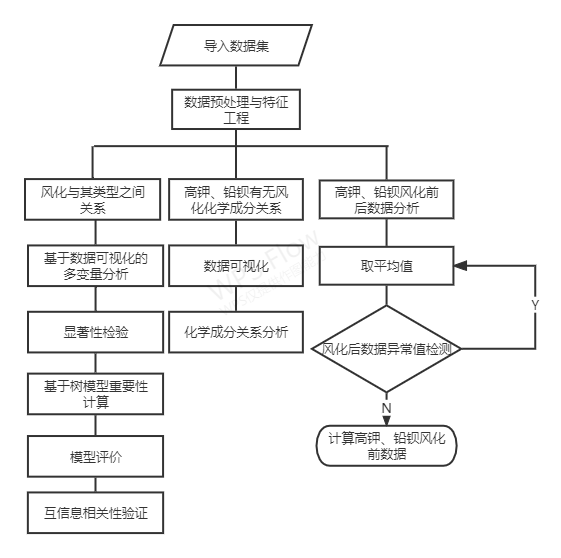
\includegraphics[width=0.95\textwidth]{1.png} %插入图片,[]中设置图片大小,{}中是图片文件名
	\caption{附录图表1} %最终文档中希望显示的图片标题
	\label{Fig.main2} %用于文内引用的标签
\end{figure}

\begin{table}[H]
	\centering
	\begin{tabular}{c c} 
		\toprule[1.5pt]
		符号 & 含义  \\ 
		\midrule[1pt]
		$i=1,i=2$ & 分别表示高钾、铅钡玻璃 \\ 
		$j$ & 表示表中从二氧化硅($SiO_2$)到二氧化硫($SO_2$)中第$j$类化学物质 \\
		$z=1,z=2$ & 分别表示风化前和风化后 \\
		$x_1,x_2,x_3,x_4$ & 分别表示纹饰、类型、颜色、风化表面 \\
		$y_j$ & 表示第$j$类化学物质的含量 \\ 
		$\overline{y_j}$ & 表示第$j$类化学物质的平均含量 \\  
		\toprule[1.5pt]
	\end{tabular}
    \caption{附录图表1}
\end{table} 



\end{document} 